%%% タイトル howtouse2
\documentclass[landscape,10pt]{ujarticle}
\special{papersize=\the\paperwidth,\the\paperheight}
\usepackage{ketpic,ketlayer}
\usepackage{ketslide}
\usepackage{amsmath,amssymb}
\usepackage{bm,enumerate}
\usepackage[dvipdfmx]{graphicx}
\usepackage{color}
\definecolor{slidecolora}{cmyk}{0.98,0.13,0,0.43}
\definecolor{slidecolorb}{cmyk}{0.2,0,0,0}
\definecolor{slidecolorc}{cmyk}{0.2,0,0,0}
\definecolor{slidecolord}{cmyk}{0.2,0,0,0}
\definecolor{slidecolore}{cmyk}{0,0,0,0.5}
\definecolor{slidecolorf}{cmyk}{0,0,0,0.5}
\definecolor{slidecolori}{cmyk}{0.98,0.13,0,0.43}
\def\setthin#1{\def\thin{#1}}
\setthin{0}
\newcommand{\slidepage}[1][s]{%
\setcounter{ketpicctra}{18}%
\if#1m \setcounter{ketpicctra}{1}\fi
\hypersetup{linkcolor=black}%

\begin{layer}{118}{0}
\putnotee{122}{-\theketpicctra.05}{\small\thepage/\pageref{pageend}}
\end{layer}\hypersetup{linkcolor=blue}

}
\usepackage[dvipdfmx]{pict2e}
\usepackage{pict2e}
\usepackage[dvipdfmx,colorlinks=true,linkcolor=blue,filecolor=blue]{hyperref}

\setmargin{25}{145}{15}{100}

\ketslideinit

\pagestyle{empty}

\begin{document}

\def\mainslidetitley{22}
\def\ketcletter{slidecolora}
\def\ketcbox{slidecolorb}
\def\ketdbox{slidecolorc}
\def\ketcframe{slidecolord}
\def\ketcshadow{slidecolore}
\def\ketdshadow{slidecolorf}
\def\slidetitlex{6}
\def\slidetitlesize{1.3}
\def\mketcletter{slidecolori}
\def\mketcbox{yellow}
\def\mketdbox{yellow}
\def\mketcframe{yellow}
\def\mslidetitlex{62}
\def\mslidetitlesize{2}

\color{black}
\normalsize\bf\boldmath
\addtocounter{page}{-1}

\def\rad{\;\mathrm{rad}}
\newcommand{\hako}[2][6mm]{\fbox{$\mathstrut$\Ctab{#1}{#2}}}
\newcommand{\dint}{\displaystyle\int}
\newcommand{\dlim}{\displaystyle\lim}
\setmargin{25}{150}{15}{100}%
\setcounter{page}{1}
%%%%%%%%%%%%%

%%%%%%%%%%%%%%%%%%%%

\newslide{KeTMathお試しパック}

\vspace*{18mm}

%%repeat=8
\slidepage
\begin{enumerate}[(1)]
\item
CTAN\verb|>|ketcindy のrepositoryでketcindy-masterをダウンロードする.
\item
HowToUseJ.pdfに従ってインストールする.
\item
タブ区切りをサポートするアプリ(Excel, OpenOfficeなど)を用意する.
\item
otamesi.zipをダウンロードして解凍する.\\
 mkanscsv.cdy, mkcard.cdy, mkscoremaxima.cdy\\
 dataフォルダ\\
   データサンプル,queans(+date).txt,students(+year).csv
\item
このスライドの6ページ以降に従って実行する.
\end{enumerate}
%%%%%%%%%%%%

%%%%%%%%%%%%%%%%%%%%

\newslide{数式の簡易記法1}

\vspace*{18mm}

%%repeat=4,para
\slidepage
\begin{itemize}
\item
文字定数(変数)は1文字とする.\vspace{-2mm}
\item
テキストにするには tx(テキスト)
\item
\Ltab{4.5zw}{分数}$\frac{a}{b}\ \Longrightarrow$\ \verb|(a)/(b)|,\ \verb|fr(a,b)| \vspace{-2mm}
\item
\Ltab{4.5zw}{掛け算}$ab\ \Longrightarrow$\ \verb|ab|\vspace{-2mm}
\item
\Ltab{4.5zw}{べき乗}$a^b\ \Longrightarrow$\ \verb|a^(b)|\vspace{-2mm}
\item
\Ltab{4.5zw}{べき乗根}$\sqrt{a},\ \sqrt[3]{a}\ \Longrightarrow$\ \verb|sq(a), sq(3,a)|\vspace{-2mm}
\item
\Ltab{4.5zw}{三角関数}$\sin x, \sin^2x\ \Longrightarrow$\ \verb|sin(x), sin(2,x)|\vspace{-2mm}
\item
\Ltab{4.5zw}{円周率}$\pi \ \Longrightarrow$\ \verb|pi(x)|\vspace{-2mm}
\item
\Ltab{4.5zw}{対数関数}$\log x, \log_a x\ \Longrightarrow$\ \verb|log(x), log(s,x)|\vspace{-2mm}
\end{itemize}
%%%%%%%%%%%%

%%%%%%%%%%%%%%%%%%%%

\newslide{数式の簡易記法2}

\vspace*{18mm}

%%repeat=4,para
\slidepage
\begin{itemize}
\item
\Ltab{4.5zw}{積分}$\dint x^2\,dx,\ \dint_a^b x^2\,dx \ \Longrightarrow$\ \verb|int()x^2dx, int(a,b)x^2dx|\vspace{-2mm}\\
\phantom{\Ltab{4.5zw}{積分}$\dint x\,dx,\ \dint_a^b x\,dx \ \Longrightarrow$}\ または \verb|int(,,x^2,x), int(a,b,x^2,x)|\vspace{-2mm}
\item
\Ltab{4.5zw}{極限}$\dlim_{x \to a}f(x) \ \Longrightarrow$\ \verb|lim(x,a)f(x)|\ または \verb|lim(x,a,f(x))|\vspace{-2mm}
\item
\Ltab{7zw}{微分・偏微分}$\dfrac{dy}{dx},\ \dfrac{\partial z}{\partial x} \ \Longrightarrow$\ \verb|diff(y,x)|, \verb|par(z,x)|
\item
\Ltab{7zw}{行列・行列式}$\begin{pmatrix}a&b\\c&d\end{pmatrix},\ \left|\begin{array}{cc}a&b\\c&d\end{array}\right|
\ \Longrightarrow$\ \verb|mat(a,b;c,d)|, \verb|det(a,b;c,d)|\vspace{-2mm}
\item
\Ltab{4.5zw}{場合分け}$\begin{cases}a&(b)\\c&(d)\end{cases} \ \Longrightarrow$\ \verb|case(a,(b);c,(d))|\vspace{-2mm}
\end{itemize}
%%%%%%%%%%%%%

%%%%%%%%%%%%%%%%%%%%

\newslide{準備}

\vspace*{18mm}

%%repeat=3
\slidepage
\begin{enumerate}[(1)]
\item
学生リスト\verb|student.csv|を作成する.\\
  番号, 名前, 登録名(姓),登録名(名),メールアドレス\\
 または\\
  番号, 学籍, 名前, ふりがな, 登録名(姓), 登録名(名), メールアドレス
\item
作業フォルダにmkanscsv.cdyとmkcard.cdyを入れる.
\item
サブフォルダ「data」を作成する.
\item
dataに次のファイルを入れる.\\
  学生リストstudent(+year).csv\\
  問題と正解のファイルqueans(+date).txt
\end{enumerate}
%%%%%%%%%%%%%

%%%%%%%%%%%%%%%%%%%%

\newslide{GCでのファイルの作成}

\vspace*{18mm}

\slidepage

\begin{layer}{120}{0}
\putnotese{50}{30}{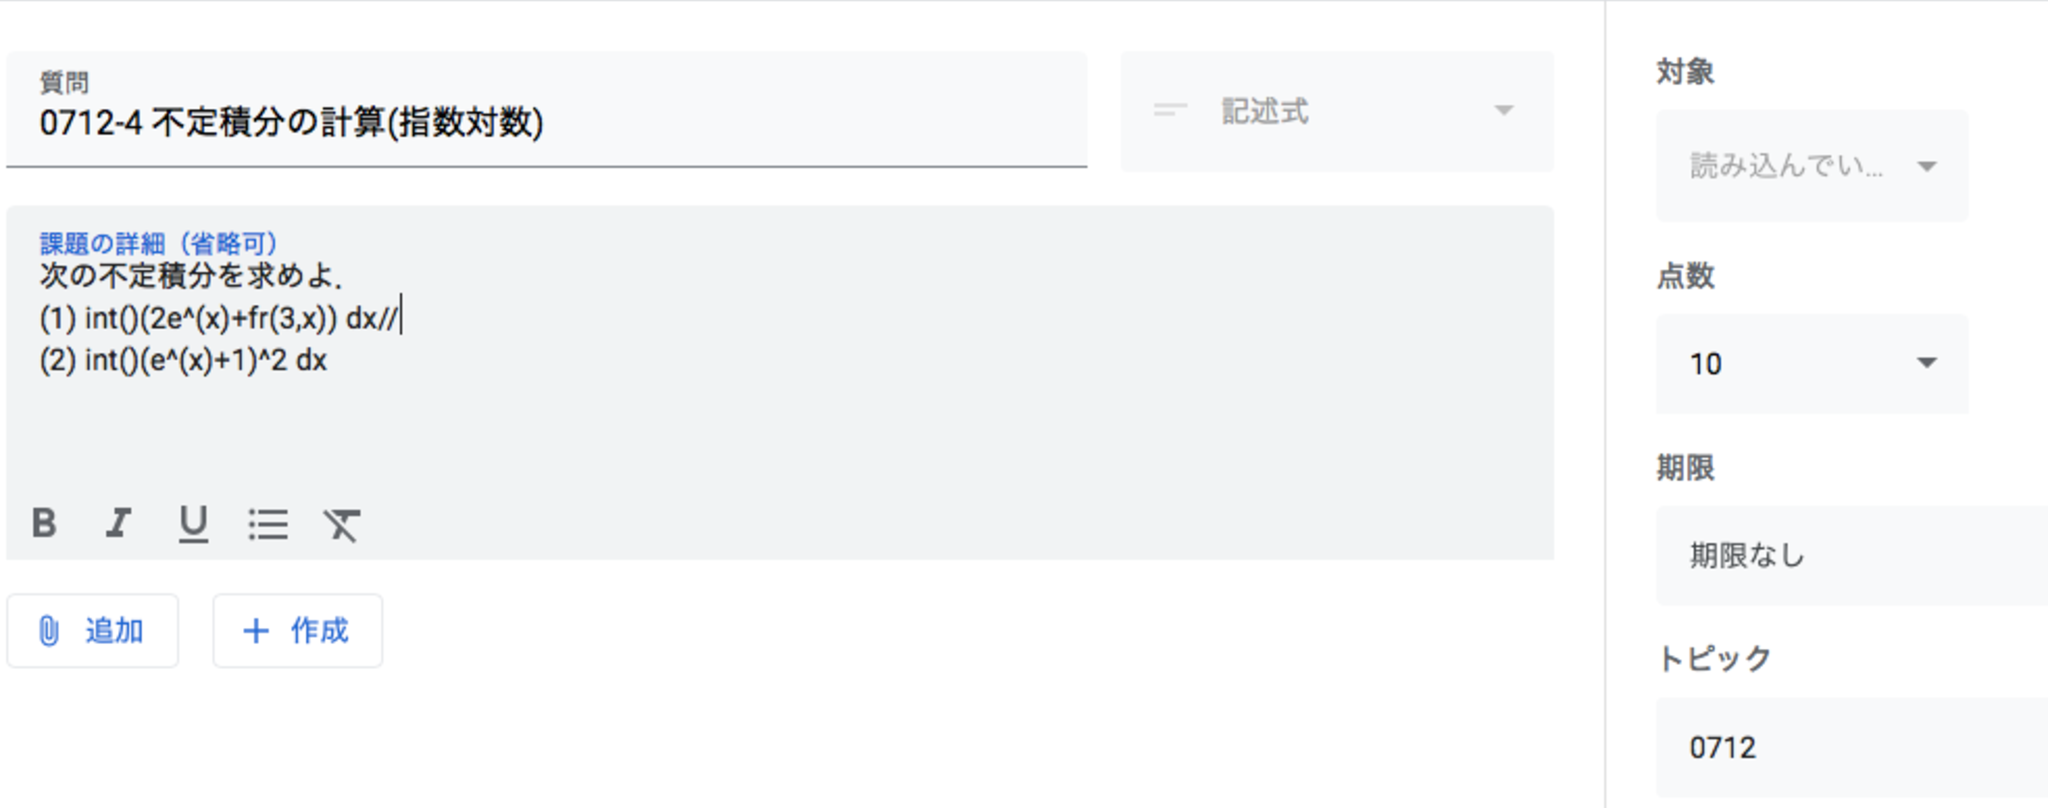
\includegraphics[bb=0.00 0.00 983.00 388.00,width=80mm]{fig/situmon.pdf}}
%%\putnotese{50}{30}{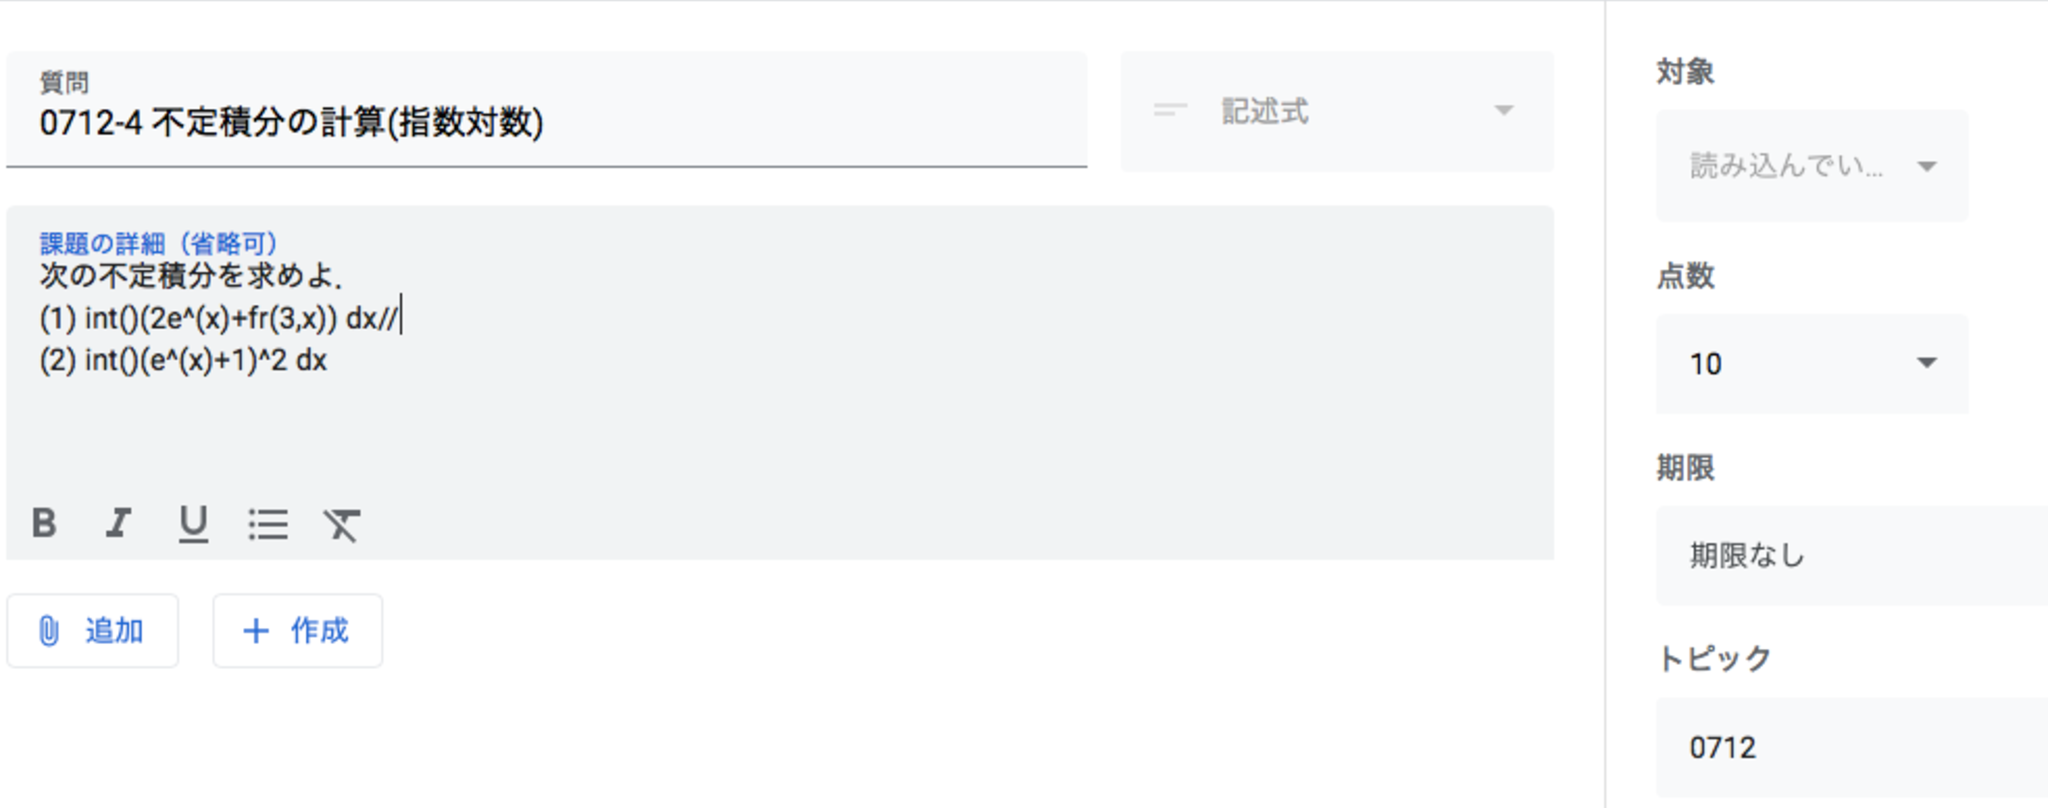
\includegraphics[bb=0.00 0.00 983.00 388.00,width=75mm]{fig/situmon.pdf}}
\end{layer}

\begin{enumerate}[(1)]
\item
「質問」で作成する.\\
 例えば,\verb|08231不定積分の公式|
\end{enumerate}
%%%%%%%%%%%%%

%%%%%%%%%%%%%%%%%%%%


\sameslide

\vspace*{18mm}

\slidepage

\begin{layer}{120}{0}
\putnotese{50}{30}{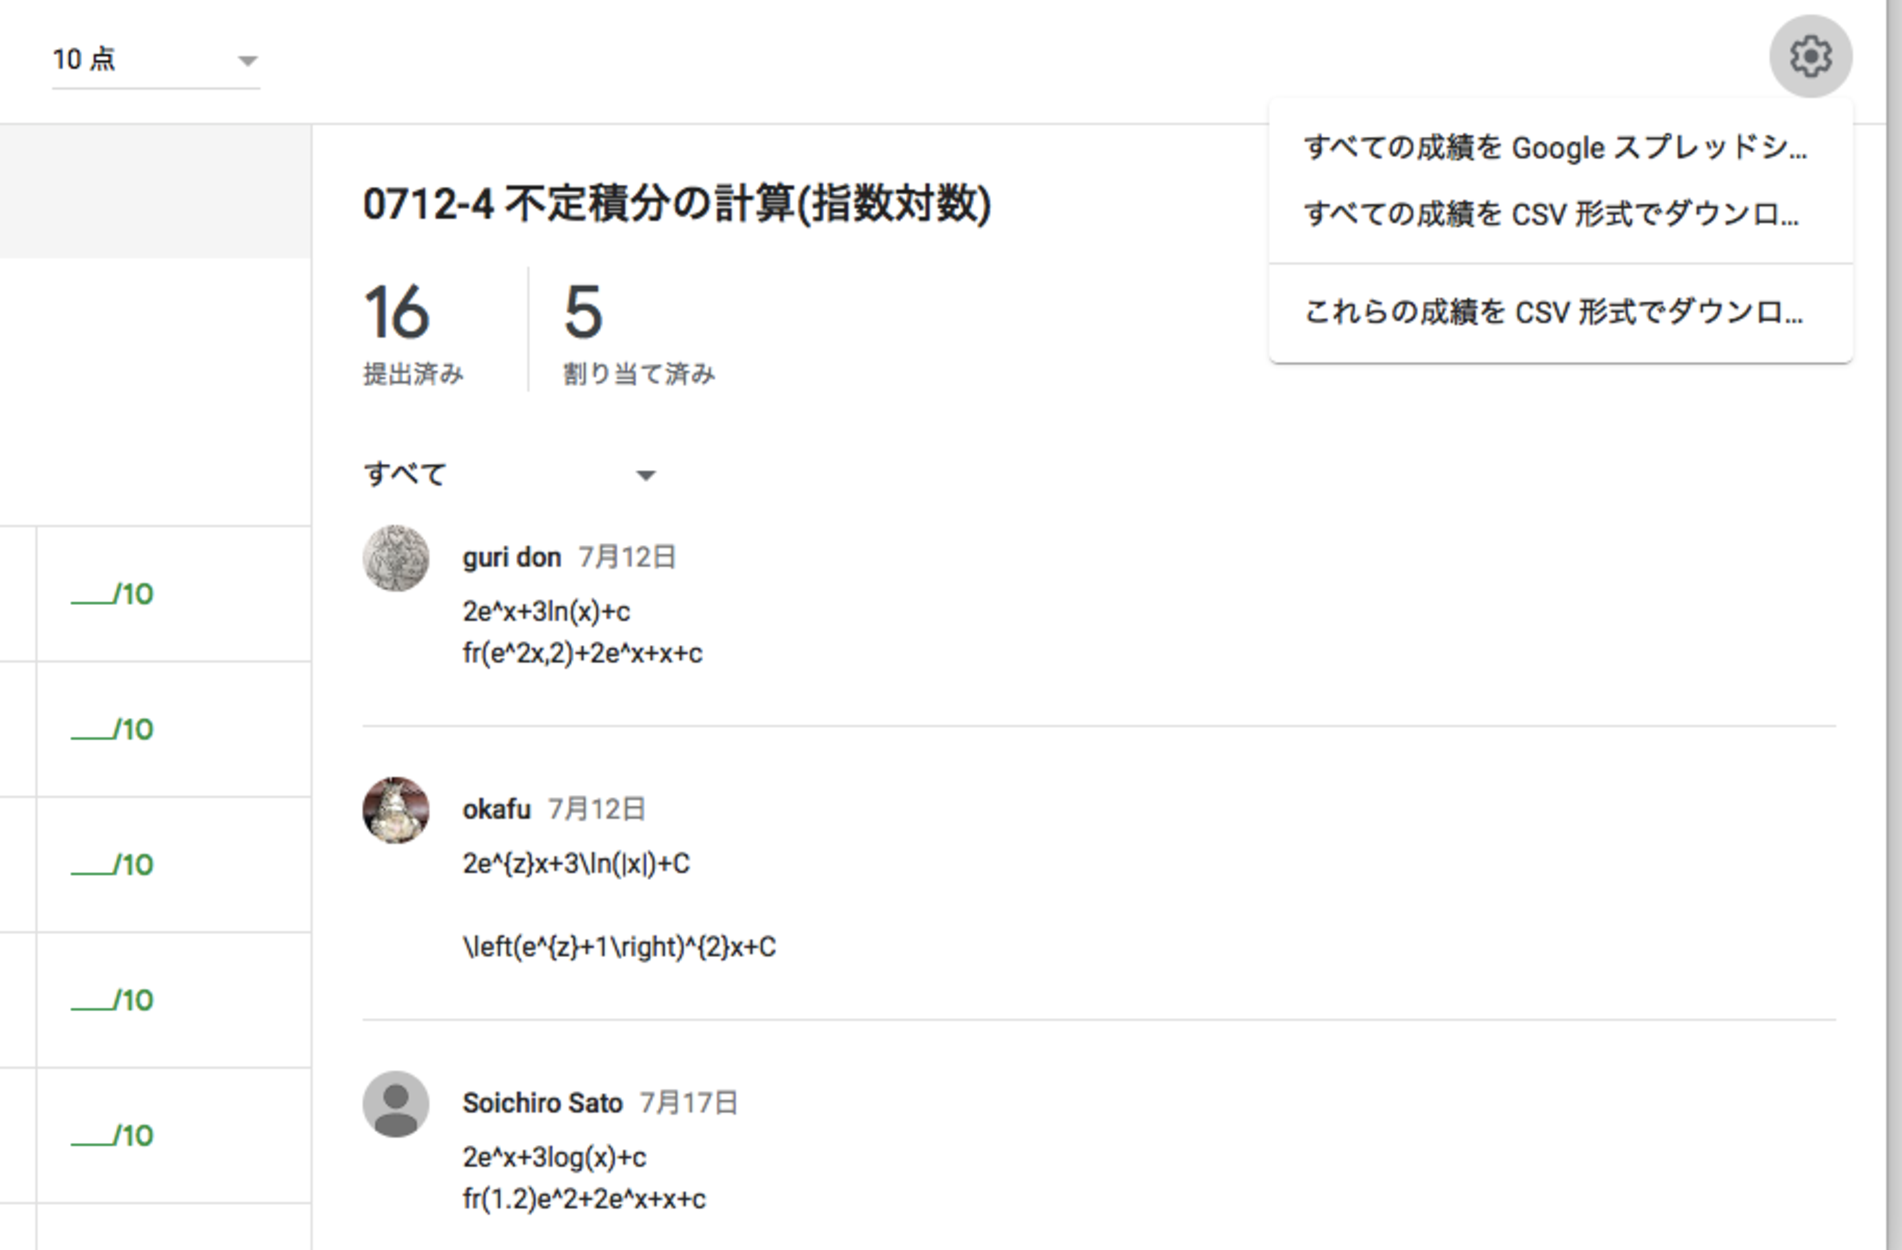
\includegraphics[bb=0.00 0.00 913.00 600.00,width=75mm]{fig/gearcsv.pdf}}
\end{layer}

\begin{enumerate}[(1)]
\item
「質問」で作成する.\\
 例えば,\verb|08231不定積分の公式|
\item
採点を選び,ギヤマークで「これらの成績をcsv形式」\\
 例えば \verb|08231不定積分の公式.csv|ができる
\end{enumerate}

\sameslide

\vspace*{18mm}

\slidepage

\begin{layer}{120}{0}
\putnotese{50}{30}{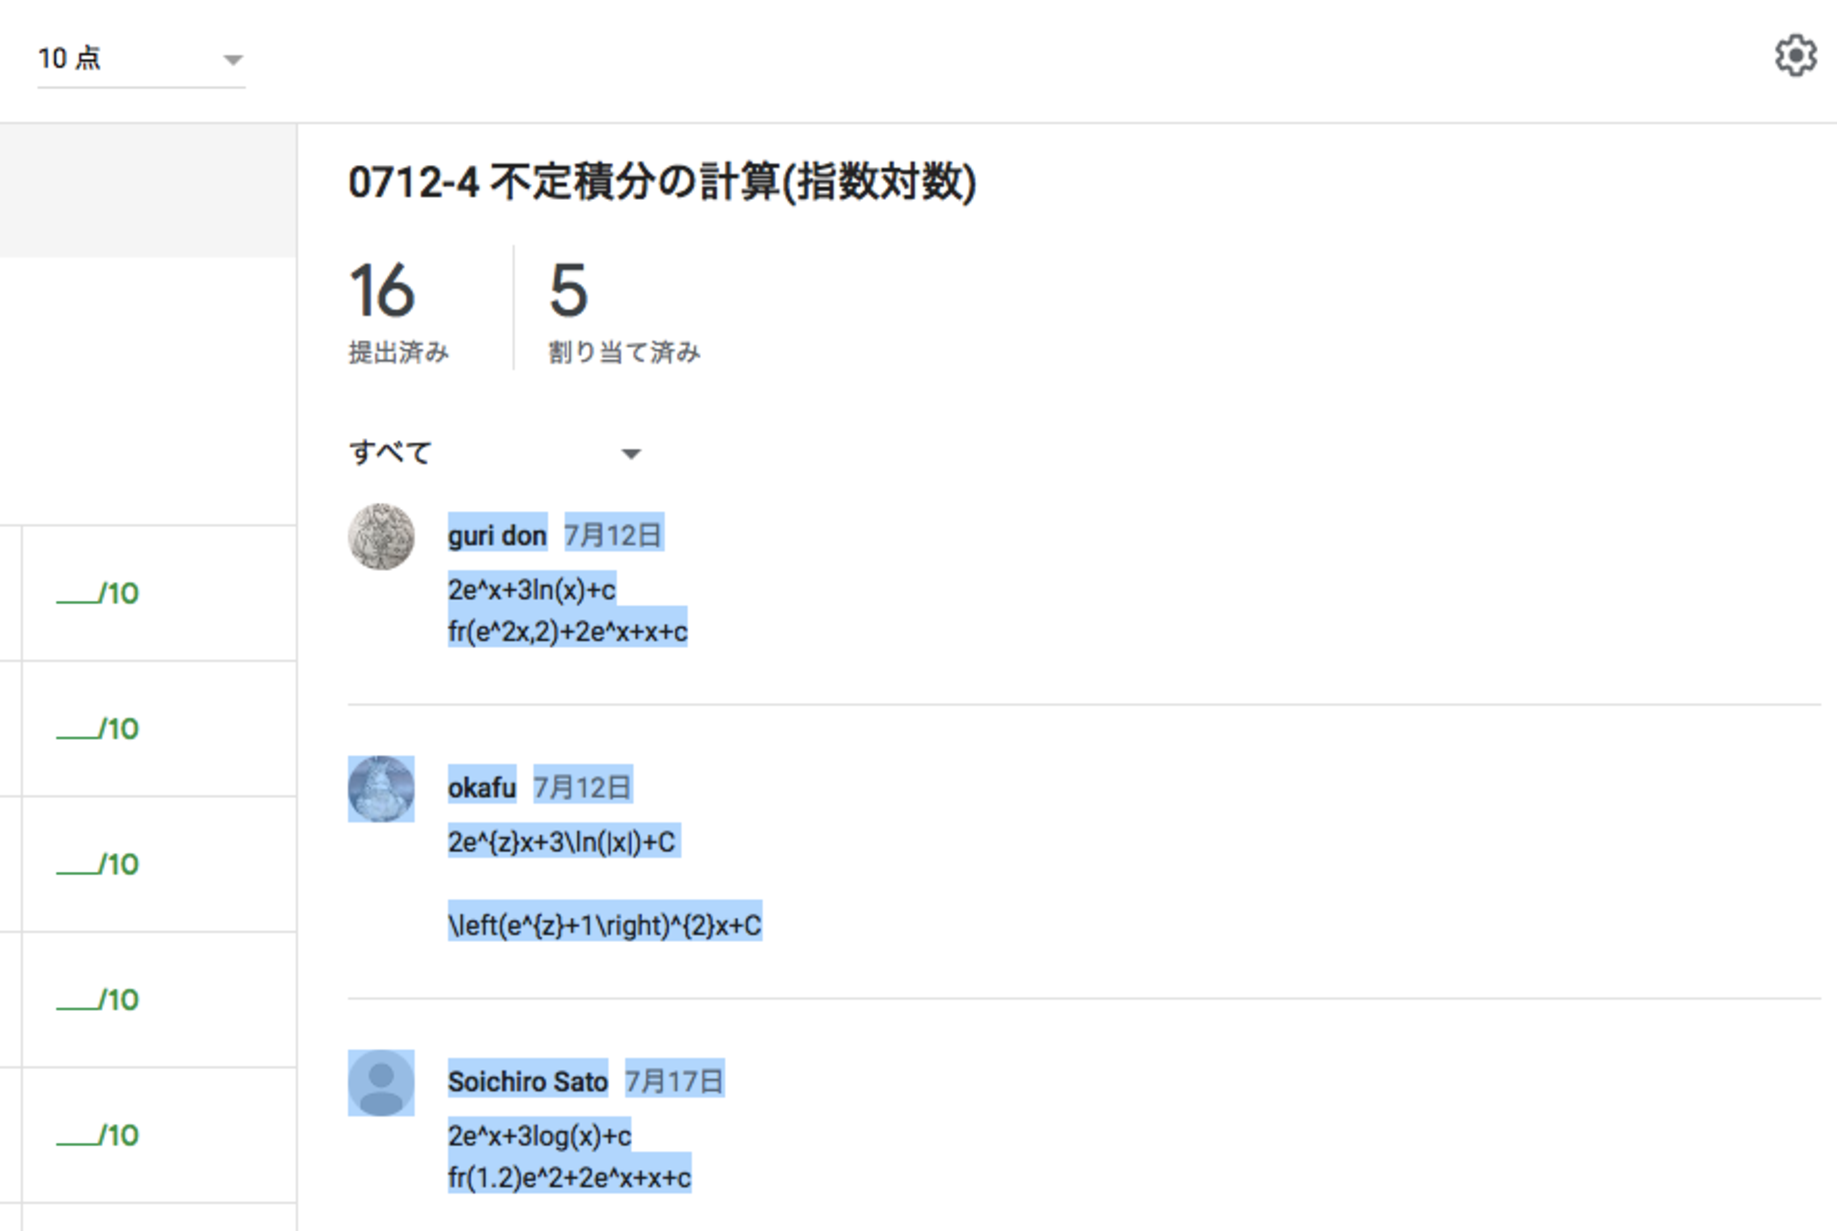
\includegraphics[bb=0.00 0.00 882.00 591.00,width=75mm]{fig/kaitou.pdf}}
\end{layer}

\begin{enumerate}[(1)]
\item
「質問」で作成する.\\
 例えば,\verb|08231不定積分の公式|
\item
採点を選び,ギヤマークで「これらの成績をcsv形式」\\
 例えば \verb|08231不定積分の公式.csv|ができる
\item
回答のすべてを選択\\
textファイルで保存\\
 例えば,\verb|08231.txt|
\item
(2)(3)のファイルを\\dataに入れる.
\end{enumerate}

\newslide{一覧ファイルの作成}

\vspace*{18mm}

%%repeat=3
\slidepage

\begin{layer}{120}{0}
\putnotese{60}{-7}{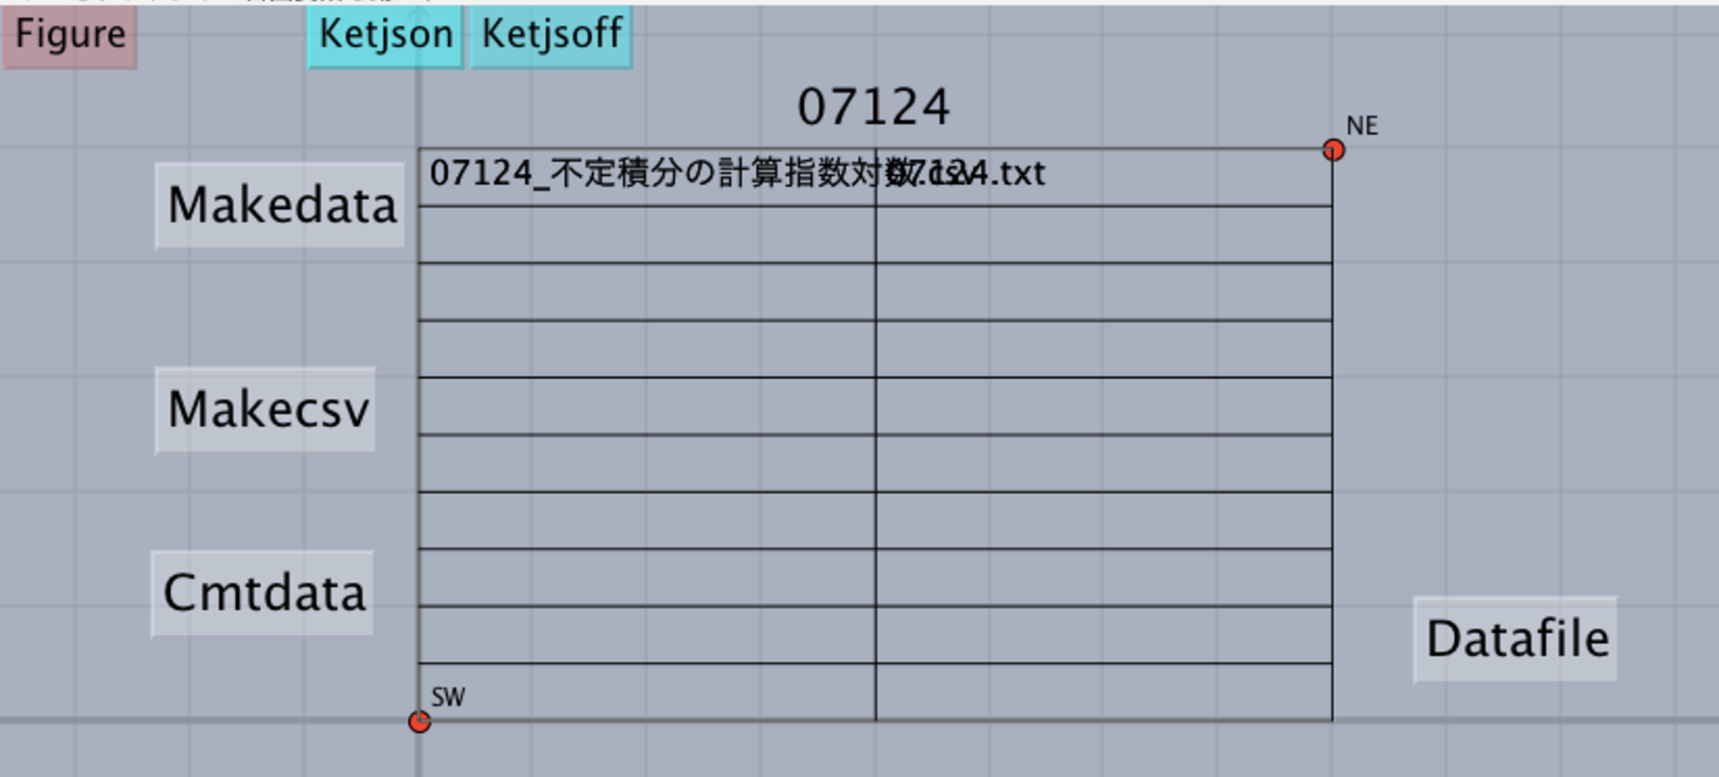
\includegraphics[bb=0.00 0.00 825.00 373.00,width=65mm]{fig/ketgcdata.pdf}}
\end{layer}

\begin{enumerate}[(1)]
\item
\verb|mkanscsv.cdy|を立ち上げる\vspace{-1mm}
\item
カーソルで枠を順に選びクリック\\
head(以下 07121とする)表示\vspace{-1mm}
\item
\verb|Mkdata, Makecsv|を押すと,次のファイルがdataにできる.\\
 \Ltab{35mm}{ans07121.csv}学生名や学生の答えを入れた一覧表(タブ区切り)\\
 \Ltab{35mm}{} ・答えは8列(修正用)と10列の両方に入る.\\
 \Ltab{35mm}{ansline07121.txt}すべてのデータを1行にしたファイル\vspace{-1mm}
\item
(2)(3)を繰り返す.\vspace{-1mm}
\item
すべてができたら,\verb|Makerec|を押すと,次のファイルがdataにできる.\\
(後でrecord07121.csvなどを作成するときに用いる)\\
 \Ltab{35mm}{rec0712.r}採点コメントを入れた1行データをタブ区切りに直す\\
 \Ltab{35mm}{reckc0712...}上の実行バッチ(record0721.csvなどすべてを作成)
\end{enumerate}
%%%%%%%%%%%%%

%%%%%%%%%%%%%%%%%%%%

\newslide{採点コメントの追加}

\vspace*{18mm}

\slidepage

\begin{layer}{120}{0}
\putnotese{65}{2}{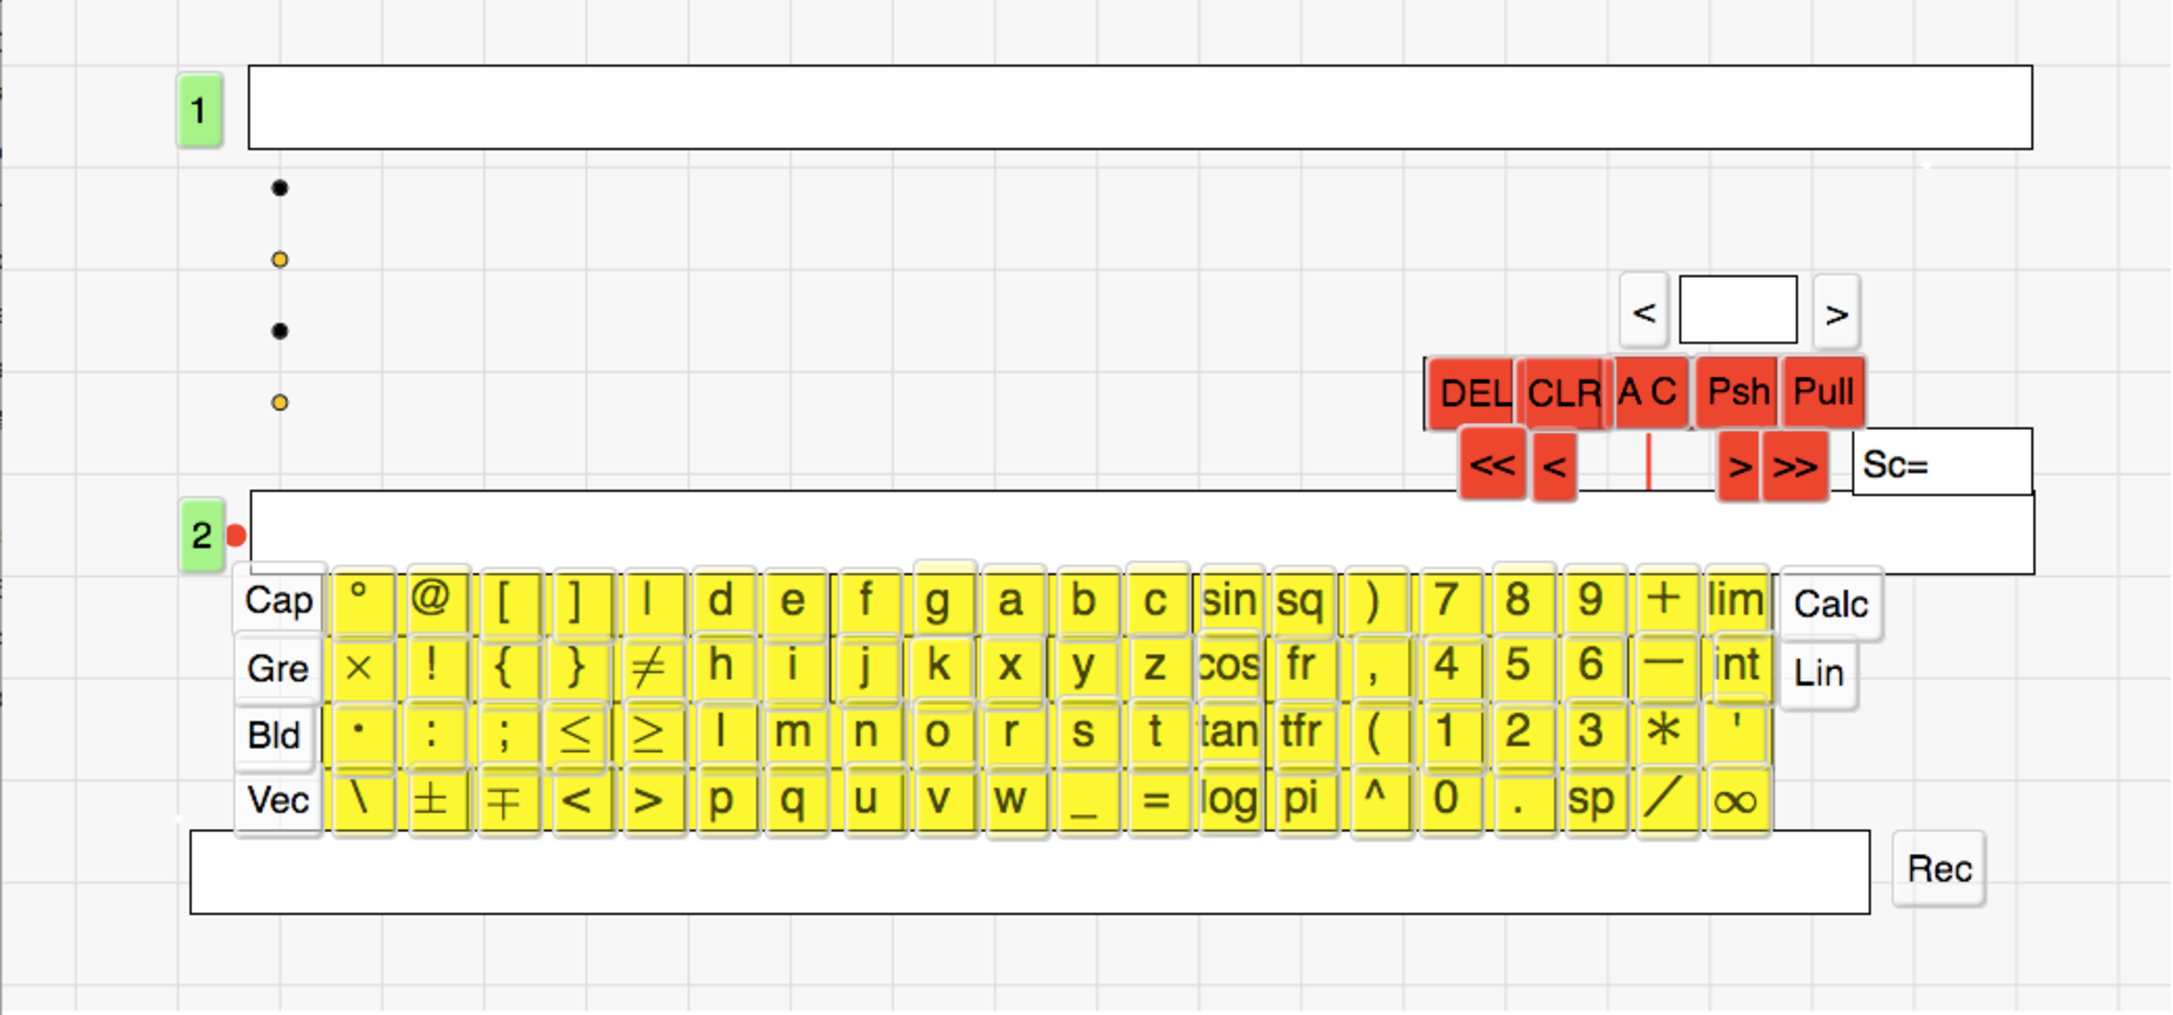
\includegraphics[bb=0.00 0.00 1043.00 487.00,width=65mm]{fig/ketmath1.pdf}}
\end{layer}

\begin{enumerate}[(1)]
\item
ketmathtoffL.htmlを立ち上げる.\vspace{-2mm}
\item
ansline07121.txtのすべてを選択\\
コピーして最下段の入力窓に入れる.\vspace{-2mm}\\
\end{enumerate}
%%%%%%%%%%%%%

%%%%%%%%%%%%%%%%%%%%


\sameslide

\vspace*{18mm}

\slidepage

\begin{layer}{120}{0}
\putnotese{65}{2}{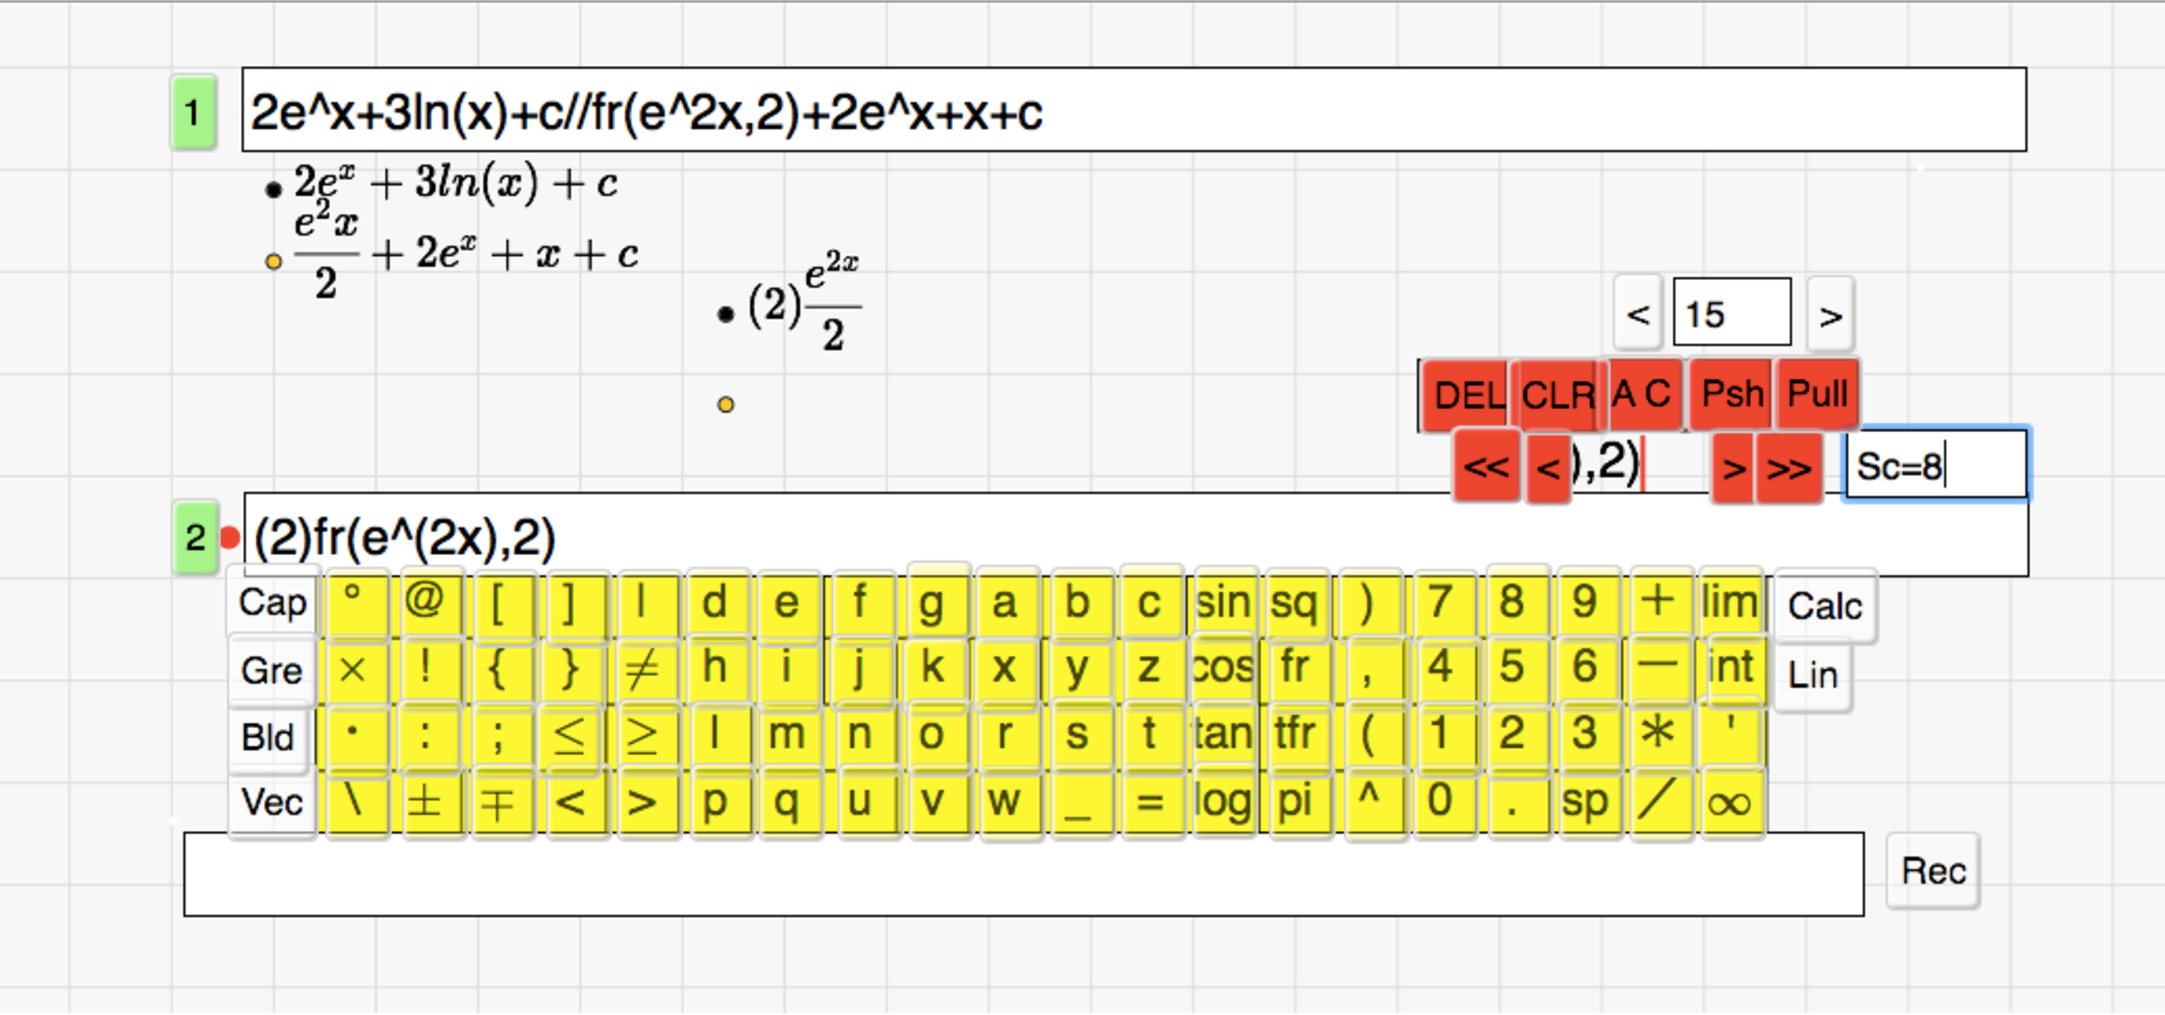
\includegraphics[bb=0.00 0.00 1043.00 487.00,width=65mm]{fig/ketmath2.pdf}}
\end{layer}

\begin{enumerate}[(1)]
\item
ketmathtoffL.htmlを立ち上げる.\vspace{-2mm}
\item
ansline07121.txtのすべてを選択\\
コピーして最下段の入力窓に入れる.\vspace{-2mm}\\
\item
<>で学生番号を変える.\vspace{-2mm}
\item
得点とコメント(2段目)を追加する.\\
 ・得点はコメントの最後に:\hspace{-2mm}:(ダブル半角コロン)をつけて書いてもよい.\vspace{-2mm}
\item
学生の答え(1段目)を入力ルールに合った数式に修正することもできる.\vspace{-2mm}
\end{enumerate}

\sameslide

\vspace*{18mm}

\slidepage

\begin{layer}{120}{0}
\putnotese{65}{2}{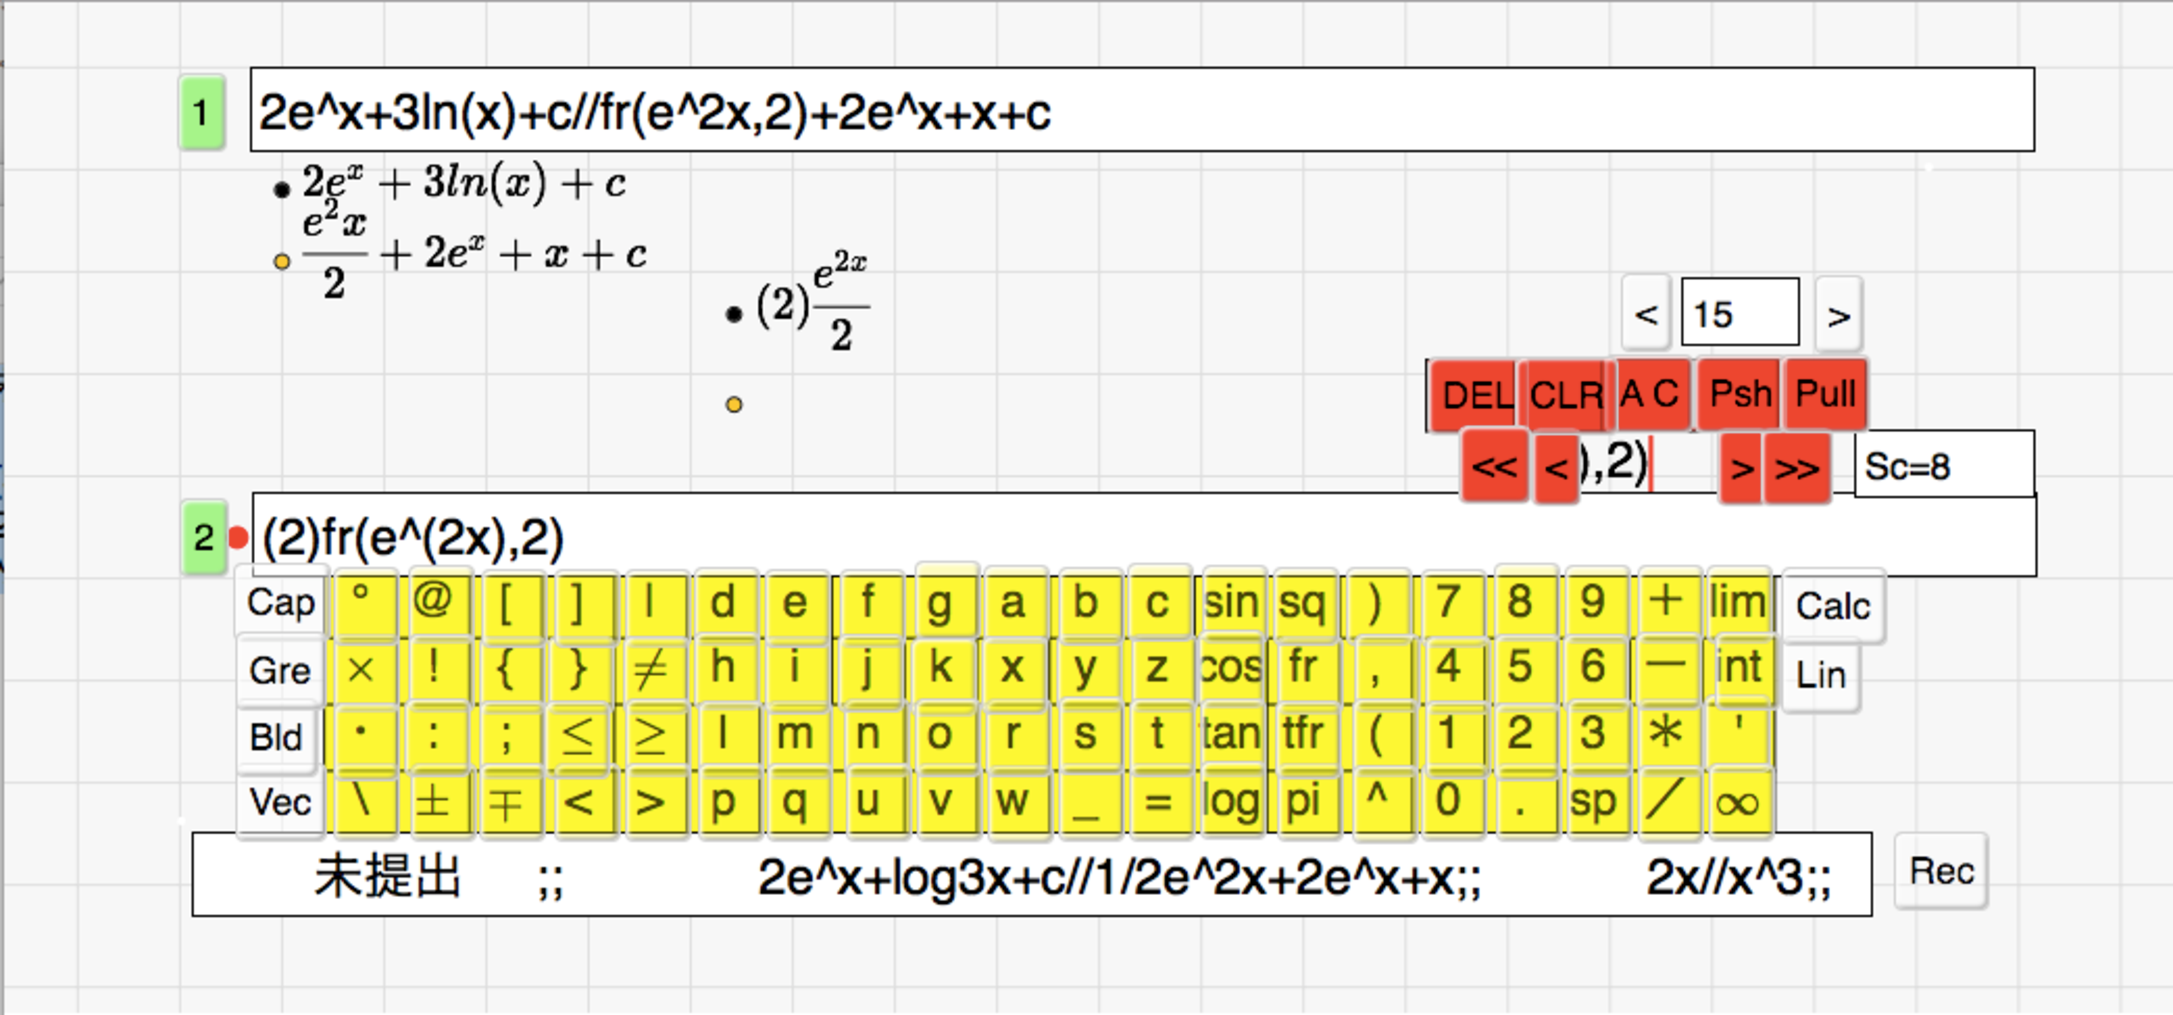
\includegraphics[bb=0.00 0.00 1043.00 487.00,width=65mm]{fig/ketmath3.pdf}}
\end{layer}

\begin{enumerate}[(1)]
\item
ketmathtoffL.htmlを立ち上げる.\vspace{-2mm}
\item
ansline07121.txtのすべてを選択\\
コピーして最下段の入力窓に入れる.\vspace{-2mm}\\
\item
<>で学生番号を変える.\vspace{-2mm}
\item
得点とコメント(2段目)を追加する.\\
 ・得点はコメントの最後に:\hspace{-2mm}:(ダブル半角コロン)をつけて書いてもよい.\vspace{-2mm}
\item
学生の答え(1段目)を入力ルールに合った数式に修正することもできる.\vspace{-2mm}
\item
Recボタンを押すと最下段にすべてのデータ(1行形式)が入る.\vspace{-2mm}
\end{enumerate}

\sameslide

\vspace*{18mm}

\slidepage

\begin{layer}{120}{0}
\putnotese{65}{2}{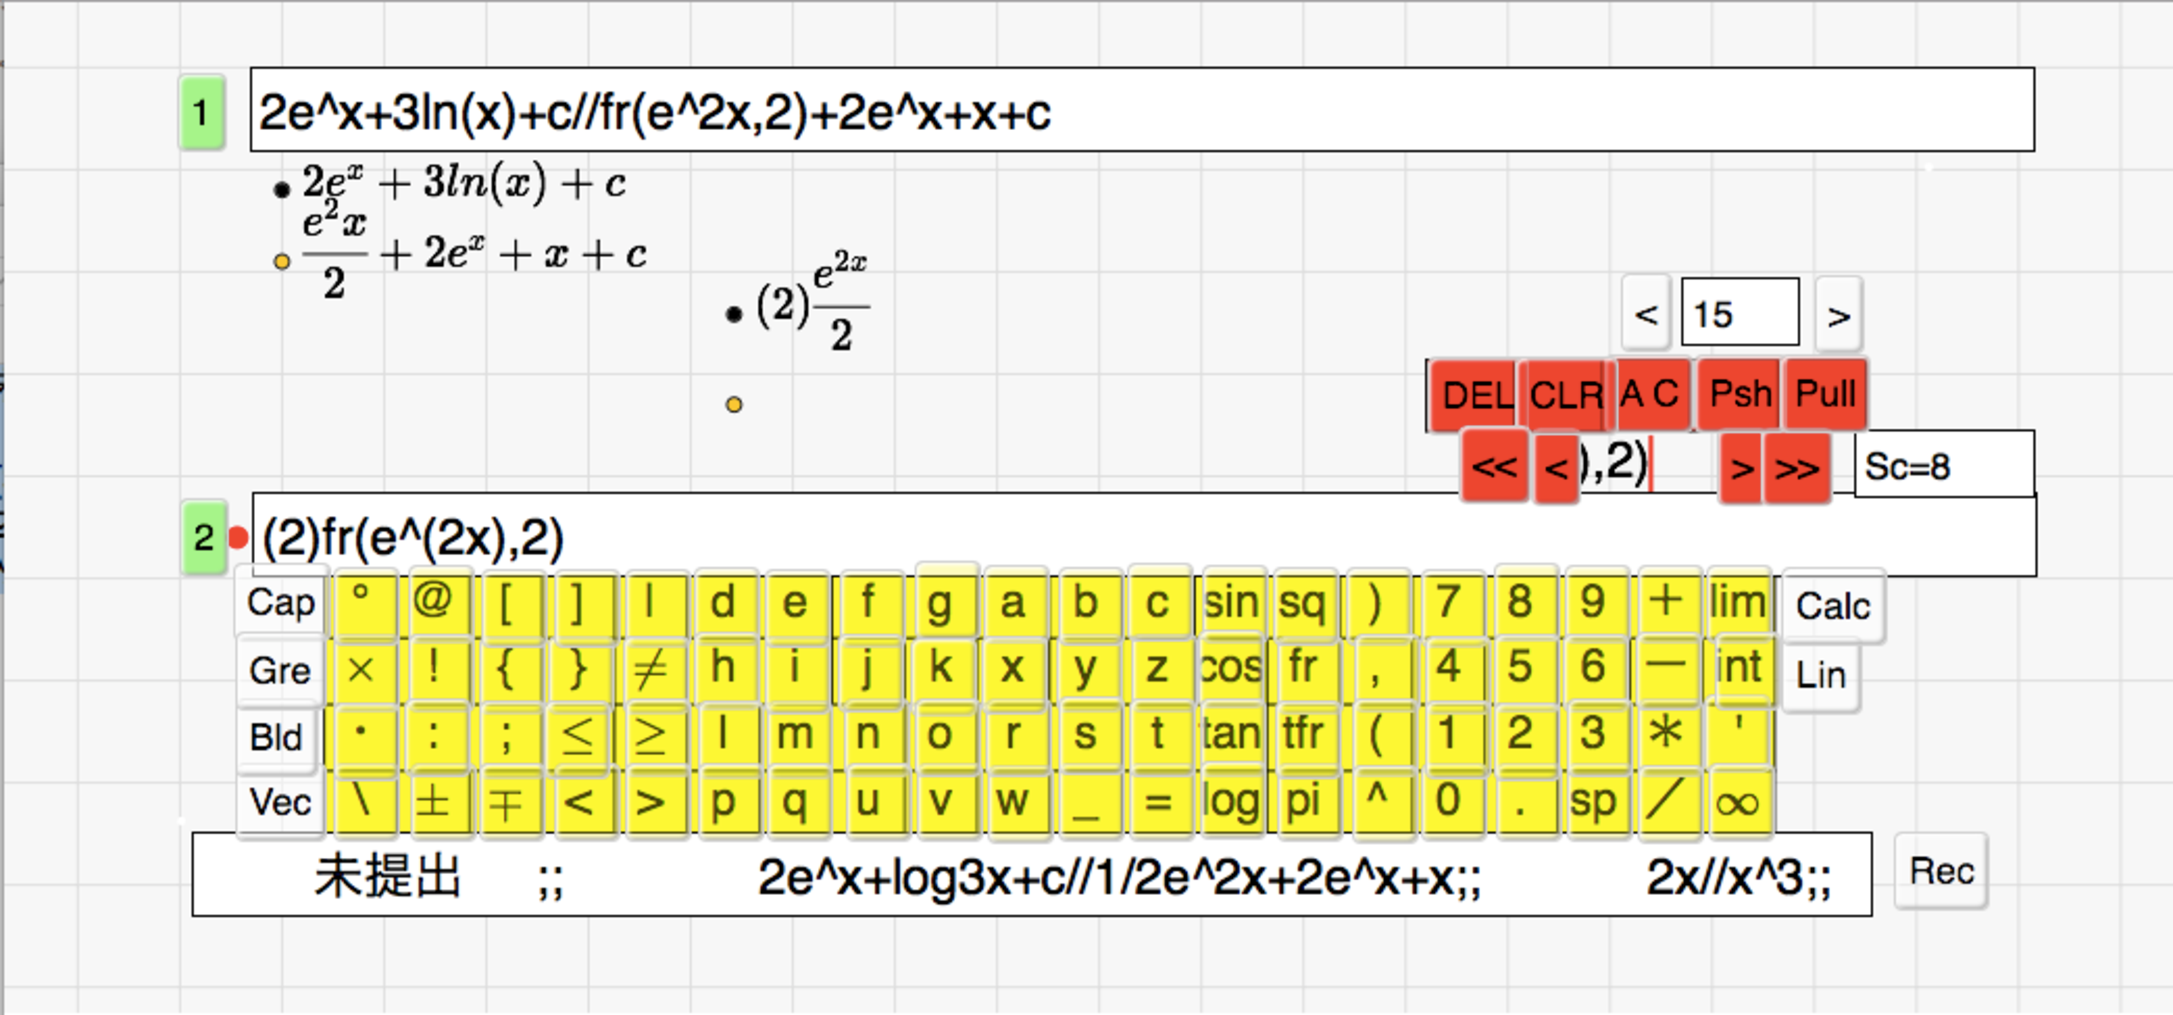
\includegraphics[bb=0.00 0.00 1043.00 487.00,width=65mm]{fig/ketmath3.pdf}}
\end{layer}

\begin{enumerate}[(1)]
\item
ketmathtoffL.htmlを立ち上げる.\vspace{-2mm}
\item
ansline07121.txtのすべてを選択\\
コピーして最下段の入力窓に入れる.\vspace{-2mm}\\
\item
<>で学生番号を変える.\vspace{-2mm}
\item
得点とコメント(2段目)を追加する.\\
 ・得点はコメントの最後に:\hspace{-2mm}:(ダブル半角コロン)をつけて書いてもよい.\vspace{-2mm}
\item
学生の答え(1段目)を入力ルールに合った数式に修正することもできる.\vspace{-2mm}
\item
Recボタンを押すと最下段にすべてのデータ(1行形式)が入る.\vspace{-2mm}
\item
すべてを選択してコピーする.\vspace{-2mm}
\item
ansline07121.txtの2行目にペーストして保存する.\vspace{-2mm}
\item
すべての問題番号で同様に行う.
\end{enumerate}

\newslide{Maximaによる採点}

\vspace*{18mm}

%%repeat=4
\slidepage
\begin{enumerate}[(1)]
\item
学生の答えをMaximaで通るように適宜修正する.\\
 Maximaでのコメントは[ ]で囲めばよい.
\item
mkscoremaximaを立ち上げて,\verb|Mkdata, Makecsv|を押す\\
 ・score(+date+no).csv(タブ区切り)ができる.\\
 ・学生の答え/正解 を計算して,次の得点を出力する.\\
    1 $\Longrightarrow$ 10,未提出 $\Longrightarrow$ 0,その他 $\Longrightarrow$ 数式をそのまま
\item
score(+date+no).csvをタブ区切りで開く.
\end{enumerate}
%%%%%%%%%%%%%

%%%%%%%%%%%%%%%%%%%%

\newslide{結果ファイル(配付)の作成}

\vspace*{18mm}

%%repeat=4
\slidepage
\begin{enumerate}[(1)]
\item
dataのreckc0712をダブルクリックするとすべての課題のcsvができる.\\
 record071121.csv, ...
\item
mkcard.cdyを立ち上げて,Makedata,Makefileを順に押す.\\
・dataにcardフォルダができる.\\
・各学生に配付する結果ファイルが入る.
\end{enumerate}
\label{pageend}\mbox{}

\end{document}
